\documentclass[12pt,a4paper,utf8]{ctexart}
\usepackage{graphicx}
\usepackage{amsmath}
\usepackage{amssymb}
\usepackage{subfig}
\usepackage{cite}
\usepackage[ntheorem]{empheq}
\usepackage{enumitem}
\usepackage{fullpage}
\usepackage{cleveref}
\usepackage{cellspace}
\usepackage{listings}
\usepackage{color}
\usepackage[top=2cm, bottom=2cm, left=2cm, right=2cm]{geometry}  
\usepackage{algorithm}  
\usepackage{algorithmicx}  
\usepackage{algpseudocode}  
\renewcommand{\algorithmicrequire}{\textbf{Input:}}  % Use Input in the format of Algorithm  
\renewcommand{\algorithmicensure}{\textbf{Output:}} % Use Output in the format of Algorithm 
\definecolor{gray}{rgb}{0.5,0.5,0.5}
\definecolor{dkgreen}{rgb}{.068,.578,.068}
\definecolor{dkpurple}{rgb}{.320,.064,.680}

% set Matlab styles
\lstset{
   language=Matlab,
   keywords={break,case,catch,continue,else,elseif,end,for,function,
      global,if,otherwise,persistent,return,switch,try,while},
   basicstyle=\small\ttfamily,
   keywordstyle=\color{blue}\bfseries,
   commentstyle=\color{dkgreen},
   stringstyle=\color{dkpurple},
   backgroundcolor=\color{white},
   tabsize=4,
   showspaces=false,
   showstringspaces=false
}

\begin{document}
\CJKfamily{zhkai}	


\begin{center}
\textbf{作业一}\\
\textbf{姓名:晏瑞然~~~~~~~~~~~~~ 学号:PB19000196~~~~~~~~~~~~~~ 日期:4.28}\\
\end{center}

\begin{center}
\fbox{
\begin{minipage}{40em}
\vspace{5cm}
\hspace{20cm}
\end{minipage}}
\end{center}
\vspace{1cm}

\begin{enumerate}
\item[第一题] \textbf{线性系统求解}  

(a),(b):

两题中生成图如下,由图可知$\omega=1.6$时收敛速度最快。

\begin{figure}[h]
   \centering
   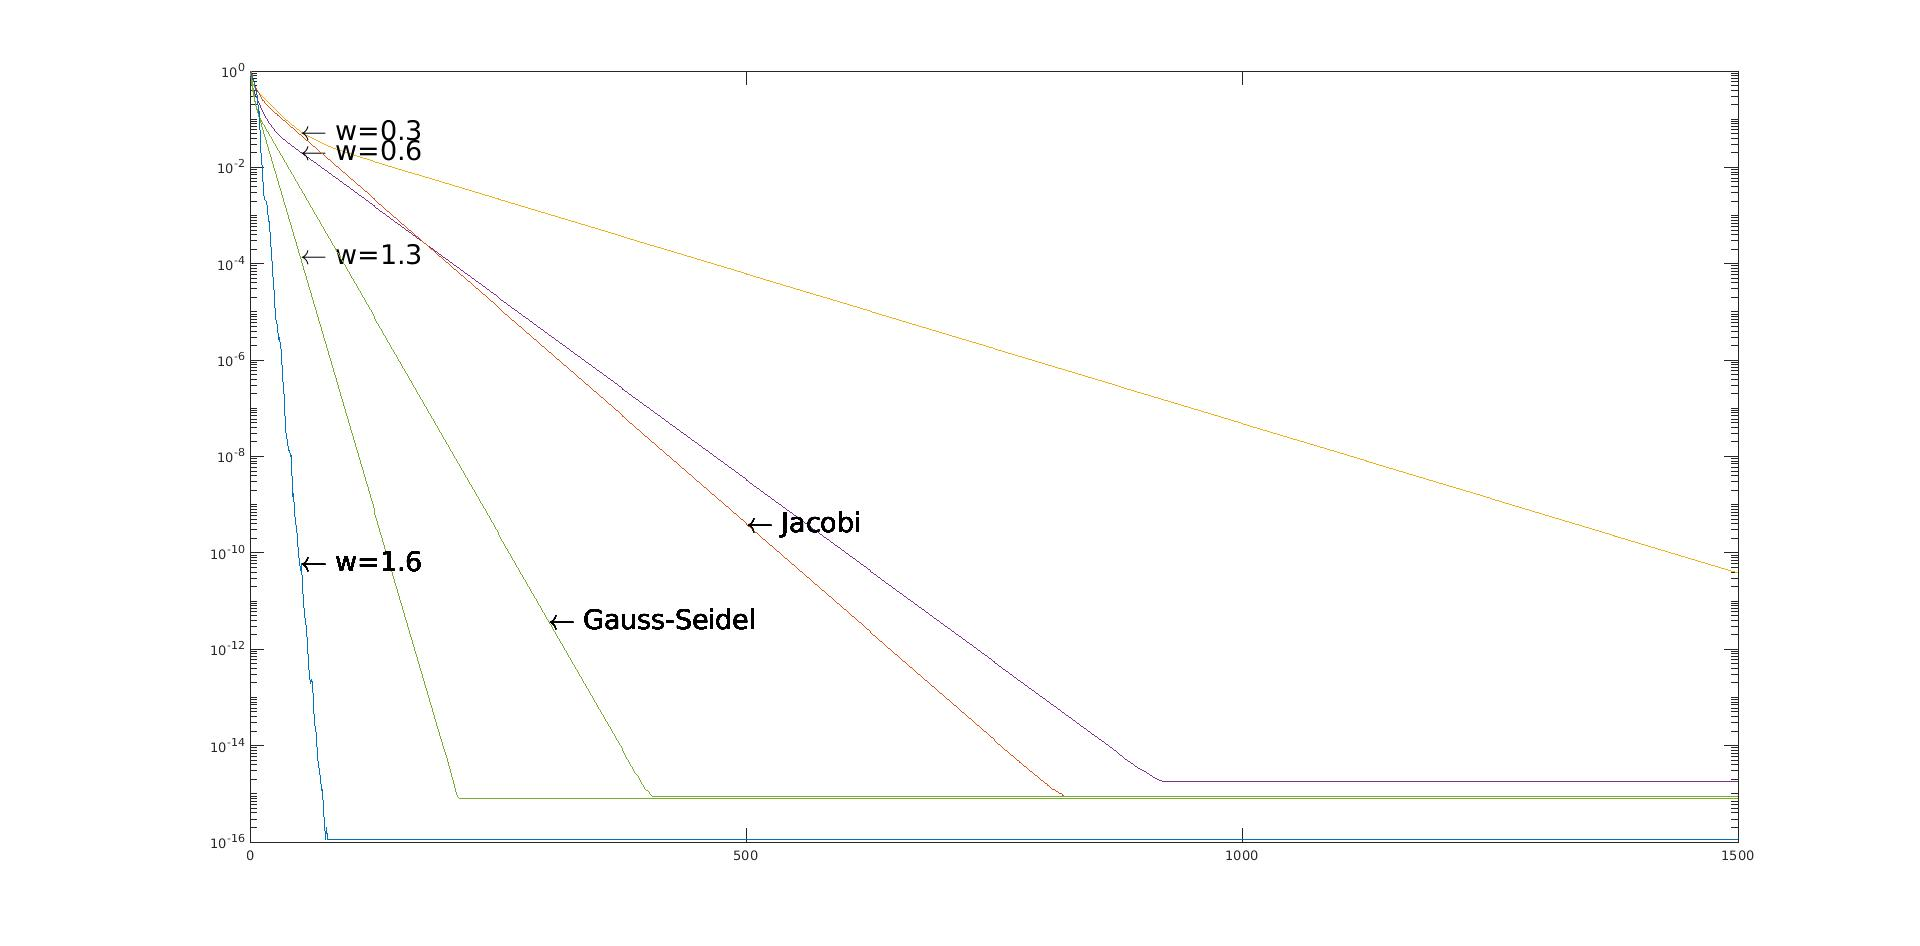
\includegraphics[width=15cm,height=8cm]{ex1_2.jpg}
   \caption{第一题(a)、(b)}
\end{figure}

(c):

程序思路:
不使用矩阵运算,直接将每次迭代用循环表达。
这样可以避免0元素的运算。

程序说明:
因为单次运算时间过短,每次统计计算10次运算的结果,除去第一次统计,统计10-1次。
实验中限制迭代次数为1500次,SOR迭代中$\omega=1.6$,所得时间单位为秒,保留4位小数。

实验数据与统计平均结果如下:

\begin{table}[htbp]

   \caption{实验数据表(除去第一次)}
	\begin{tabular}{ | c | c | c | c | c | c | c | c | c | c |}
		\hline
		实验次数 	            & 2 & 3 & 4 & 5 & 6 & 7 & 8 & 9 & 10 \\ 
		\hline
		Jacobi(未加速) 	      & 0.0079 & 0.0048 & 0.0061 & 0.0050 & 0.0076 & 0.0056 & 0.0053 & 0.0055 & 0.0049 \\ 
		\hline 
		Jacobi(加速)            & 0.0040 & 0.0038 & 0.0041 & 0.0038 & 0.0041 & 0.0038 & 0.0040 & 0.0039 & 0.0041 \\ 
		\hline 
      Gauss(未加速) 	         & 0.0500 & 0.0315 & 0.0399 & 0.0351 & 0.0436 & 0.0427 & 0.0345 & 0.0361 & 0.0333 \\ 
		\hline 
		Gauss(加速)             & 0.0022 & 0.0022 & 0.0022 & 0.0021 & 0.0021 & 0.0020 & 0.0021 & 0.0021 & 0.0021 \\ 
		\hline 
      SOR(未加速)  	         & 0.0323 & 0.0297 & 0.0321 & 0.0344 & 0.0367 & 0.0283 & 0.0409 & 0.0294 & 0.0308 \\ 
		\hline 
		SOR(加速)               & 0.0026 & 0.0026 & 0.0029 & 0.0032 & 0.0027 & 0.0025 & 0.0025 & 0.0025 & 0.0026 \\ 
		\hline 
	\end{tabular}
\end{table}


\begin{table}[htbp]
   \centering
   \caption{统计平均结果}
	\begin{tabular}{ | c | c | c |}
		\hline
			            & 未加速 	& 加速	 \\ 
		\hline
		Jacobi 	      & 0.0059	& 0.0040		 \\ 
		\hline 
		Gauss-Seidel   & 0.0354 & 0.0021		 \\ 
      \hline 
		SOR            & 0.0327 & 0.0027		 \\
		\hline 
	\end{tabular}
\end{table}

数据解释:
可以看出Guass与SOR迭代速度优化效果明显,因为矩阵运算中这两种方法都要通过解一个线性系统来进行迭代;
而Jacobi方法矩阵迭代与加速后的迭代唯一的区别就是加速迭代去除了非零元素的计算。
本题中矩阵阶数过低故加速效果不算明显,只有微弱提升。


MATLAB程序如下:

主函数:
\begin{lstlisting}[frame=single]
% ex1.a.b
% 初始化参数
aaa = ones(10,1);
bbb = [-aaa,aaa*2,-aaa];
A = spdiags(bbb,[-1 0 1],10,10);
b = [2;-2;2;-1;0;0;1;-2;2;-2];
x_exact = [1;0;1;0;0;0;0;-1;0;-1];
% 初始化3×2时间表
timeList = zeros(3,2);
% J method
J(A,b,x_exact);
% G method
G(A,b,x_exact);
% S method
w=[0.3 0.6 1.3 1.6];
for i=1:4
    S(A,b,x_exact,w(i));
end

%ex1.c
%迭代次数:1500,Sor迭代w=1.6
T=zeros(10,1);
% 计算未加速Jabobi迭代所用时间
for i =1:10
    [~,T(i)]=J(A,b,x_exact);
end
timeList(1,1) = sum(T)-T(1);
% 计算未加速Guass迭代所用时间
for i =1:10
    [~,T(i)]=G(A,b,x_exact);
end
timeList(2,1) = sum(T)-T(1);
% 计算未加速SOR迭代所用时间
for i =1:10
    [~,T(i)]=S(A,b,x_exact,1.6);
end
timeList(3,1) = sum(T)-T(1);
% 计算加速Jabobi迭代所用时间
for i =1:10
    [~,T(i)]=J2(A,b,x_exact);
end
timeList(1,2) = sum(T)-T(1);
% 计算加速Guass迭代所用时间
for i =1:10
    [~,T(i)]=G2(A,b,x_exact);
end
timeList(2,2) = sum(T)-T(1);
% 计算加速SOR迭代所用时间
for i =1:10
    [~,T(i)]=S2(A,b,x_exact,1.6);
end
timeList(3,2) = sum(T)-T(1);
% 打印timeList
timeList
\end{lstlisting}
各子函数:
\begin{lstlisting}[frame=single]
function [x,time] = J(A,b,x_exact)
%J 使用Jacobi迭代求解线性系统,不加速

% 初始化参数
% 对角矩阵的逆可以由对角线上元素取倒数得到
D_inverse = diag(diag(1./A));
R = eye(size(A)) - D_inverse*A;
g = D_inverse*b;
err = zeros(1500,1);
x = eye(size(b));
tic % 开始计时
for i=1:1500
   err(i) = max(abs(x-x_exact)); % 记录迭代过程中每个迭代值的误差
   x = R*x+g; % 迭代公式
end
time = toc; % 结束计时
% 画图
a = 1:1500;
semilogy(a,err)
s = '\leftarrow Jacobi';
text(500,err(500),s,'FontSize',20)
hold on
end
\end{lstlisting}

\begin{lstlisting}[frame=single]
function [x2,time] = J2(A,b,x_exact)
%J2 使用Jacobi迭代求解线性系统,加速

% 初始化参数
D = diag(A);
D_inv = 1./D;
err = zeros(1500,1);
x2 = eye(size(b));
xsize=size(b,1);
tic % 开始计时
for i=1:1500
   x1 = x2;
   err(i)=max(abs(x2-x_exact));
   % 稀疏矩阵优化迭代
   x2(1)=D_inv(1)*(b(1)+x1(2));
   for j=(1+1):(size(b,1)-1)
      x2(j)=D_inv(j)*(b(j)+x1(j-1)+x1(j+1));
   end
   x2(xsize) = D_inv(xsize)*(b(xsize)+x1(xsize-1));
end
time = toc;% 停止计时
err(1500);
end
\end{lstlisting}

\begin{lstlisting}[frame=single]
function [x,time] = G(A,b,x_exact)
%G 使用Gauss-Seidel迭代求解线性系统,不加速

% 初始化参数
D = diag(diag(A));
L = tril(A)-diag(diag(A));
U = triu(A) - diag(diag(A));
err = zeros(1500,1);
x = eye(size(b));
tic % 开始计时
for i=1:1500
      err(i) = max(abs(x-x_exact));% 记录迭代过程中每个迭代值的误差
      x = (D+L)\(-U*x+b);% 迭代公式
end
time = toc;% 停止计时
% 画图
a = 1:1500;
semilogy(a,err)
s = '\leftarrow Gauss-Seidel';
text(300,err(300),s,'FontSize',20)
hold on
end
\end{lstlisting}

\begin{lstlisting}[frame=single]
function [x,time] = G2(A,b,x_exact)
%G2 使用Gauss-Seidel迭代求解线性系统,加速

% 初始化参数
D = diag(A);
D_inv = 1./D;
err = zeros(1500,1);
x = eye(size(b));
tic % 开始计时
for i=1:1500
   err(i)=max(abs(x-x_exact));% 记录误差
   % 稀疏矩阵迭代公式
   x(1)=D_inv(1)*(b(1)+x(2));
   for j=(1+1):(size(b,1)-1)
      x(j)=D_inv(j)*(b(j)+x( j-1)+x(j+1));
   end
   x(size(b,1))=D_inv(size(b,1))*(b(size(b,1))+x(size(b,1)-1));
end
time = toc;% 停止计时
err(1500);
end
\end{lstlisting}

\begin{lstlisting}[frame=single]
function [x,time] = S(A,b,x_exact,w)
%S 使用Sor迭代求解线性系统,不加速

% 初始化参数
D = diag(diag(A));
L = tril(A)-diag(diag(A));
U = triu(A) - diag(diag(A));
D_inverse = diag(diag(1./A));
L_tilde = -D_inverse*L;
U_tilde = -D_inverse*U;
g = D_inverse*b;

err = zeros(1500,1);
x = eye(size(b));
tic % 开始计时
for i=1:1500
   err(i) = max(abs(x-x_exact)); % 记录误差
   %if err(i)< 1e-15
   %    break;
   %end
   x = (eye(size(A))-w.*L_tilde)\...
   (((1-w).*eye(size(A))+w.*U_tilde)*x+w.*g); % 迭代公式
end
time = toc;% 停止计时
% 画图
a = 1:1500;
semilogy(a,err)
s = ['\leftarrow w=',num2str(w)];
text(50,err(50),s,'FontSize',20)
hold on

end
\end{lstlisting}

\begin{lstlisting}[frame=single]
function [x,time] = S2(A,b,x_exact,w)
%S2 使用Sor迭代求解线性系统,加速
% 初始化参数
D = diag(A);
D_inv = 1./D;
err = zeros(1500,1);
x = eye(size(b));
xsize=size(b,1);
tic % 开始计时
for i=1:1500
   err(i)=max(abs(x-x_exact));% 记录误差
   % 稀疏矩阵优化迭代
   x(1)=(1-w)*x(1)+w*D_inv(1)*(b(1)+x(2));
   for j=(1+1):(size(b,1)-1)
      x(j)=(1-w)*x(j)+w*D_inv(j)*(b(j)+x(j-1)+x(j+1));
   end
x(xsize) = (1-w)*x(xsize)+w*D_inv(xsize)* ...
(b(xsize)+x(xsize-1));
end
time = toc;% 停止计时
err(1500);
end
\end{lstlisting}

\newpage
\item[第二题]\textbf{Newton法求解方程}

(a)、(b):

程序思路:
选取初始值$x_l=-1.5,x_m=0.5,x_r=3$,进行牛顿迭代。
在迭代过程中,每生成3个迭代值,用$x_{k+2}$代替精确解计算
$\log(|x_{k+1}-x_{k+2}|),\log(|x_{k+1}-x_{k+2}|)$,
再由每两组上述值计算斜率,即为迭代的阶数。

程序说明:
$x$为不同初始值得到的解。
$x(i)\_list$为上述解得到的迭代过程,i可以取$l,m,r$,分别代表三个解的迭代过程。
$n(i)$为得到上述迭代估算的阶的过程,其最后一个元素即为估算的阶。

程序结果:

程序结果如下,由结果可以看出三个解分别是
$x_l=-0.732,x_m=1,x_r=2.732$,
阶分别为$n_l=2,n_m=3,n_r=2$。

\begin{lstlisting}[frame=single]
   x =

   -0.732050807568877
 
 
 xl_list =
 
   -1.500000000000000
   -0.984126984126984
   -0.773163127830252
   -0.733437807950018
   -0.732052470495501
   -0.732050807571272
   -0.732050807568877
 
 
 nl =
 
    1.568545332745191
    1.856274573297303
    1.984324400495861
    1.999720993874996
 
 
 x =
 
      1
 
 
 xm_list =
 
    0.500000000000000
    1.111111111111111
    0.999074074074074
    1.000000000529222
    1.000000000000000
 
 
 nm =
 
    3.192460317189232
    3.002594709561758
 
 
 x =
 
    2.732050807568877
 
 
 xr_list =
 
    3.000000000000000
    2.777777777777778
    2.733756613756614
    2.732053321730378
    2.732050807574352
    2.732050807568877
 
 
 nr =
 
    1.845924079368328
    1.982116998528189
    1.999631420917110
\end{lstlisting}

(c):

确实出现了阶比2大的现象,出现原因如下:

Newton法对应于$f(x)=0$的迭代方程为$\varphi (x)=x-\frac{f(x)}{f'(x)}$。

对$\varphi (x)$求导得:

$\varphi' (x)=\frac{f(x)f''(x)}{(f'(x))^2}$

$\varphi'' (x)=\frac{(f'(x)f''(x)+f'''(x)f(x))f'(x)^2-2f'(x)f(x)f''(x)^2}{(f'(x))^4}$

...

设真实解为$\alpha$本题中$\alpha=1$,该解十分特殊,因为此解同时满足$f(\alpha)=0,f''(\alpha)=0$。
将$\alpha$带入$\varphi (x)$的各阶导数,得:

$\varphi (\alpha)=\alpha,\varphi' (\alpha)=0,\varphi'' (\alpha)=0,\varphi''' (\alpha)\neq 0$

故:

$\quad x_{k+1}-\alpha \\
= \varphi (x_k)-\varphi (\alpha)\\
=\varphi (\alpha)+(x_k-\alpha)\varphi' (\alpha)+\frac{(x_k-\alpha)^2}{2!}\varphi'' (\alpha)+\frac{(x_k-\alpha)^3}{3!}\varphi''' (\xi )-\varphi (\alpha) \\
=\frac{(x_k-\alpha)^3}{3!}\varphi''' (\xi )$

$\Rightarrow \lim_{k \to \infty} \frac{|x_{k+1}-\alpha |}{|x_k-\alpha |^3}=\frac{\varphi''' (\alpha)}{3!} $

此时,牛顿迭代的阶变为3阶。

MATLAB程序如下:
\begin{lstlisting}[frame=single]
format long
% 选定初始值
xl0=-1.5;
xm0=0.5;
xr0=3;
% 多项式系数
a0=[1,-3,0,2];
% 多项式导数的系数
a1=[3,-6,0];
m=10;%迭代次数
% 求解第一个解
err=[];
xl_list=xl0;
x=xl0;
nl=[];% 创建一个阶的列表,记录每次迭代得到的阶
for i=1:m
   x1=x-(a0(1)*x^3+a0(2)*x^2+a0(3)*x+a0(4)) ... 
   /(a1(1)*x^2+a1(2)*x+a1(3));% 迭代公式
   % 两次迭代值误差小于给定值时停止迭代
   if abs(x1-x)<=1e-15
      break
   end
   err=[err;(x1-x)];% 将本次迭代的误差加入误差列表
   if i>2
      % 计算求阶时所用系数,用i+2次迭代代替真实值
      loge_k_0=log10(abs(err(i-2)+err(i-1)));
      loge_k_1=log10(abs(err(i-1)+err(i)));
      loge_kplus1_0=log10(abs(err(i-1)));
      loge_kplus1_1=log10(abs(err(i)));
      % 求阶并加入阶的列表
      nl=[nl;(loge_kplus1_0-loge_kplus1_1)/(loge_k_0-loge_k_1)];
   end
   xl_list = [xl_list;x1];
   x=x1;
end
x
xl_list
%err;
nl
% 求解第二个解,与上操作相同
err=[];
xm_list=xm0;
x=xm0;
nm=[];
for i=1:m
   x1=x-(a0(1)*x^3+a0(2)*x^2+a0(3)*x+a0(4)) ... 
   /(a1(1)*x^2+a1(2)*x+a1(3));
   if abs(x1-x)<=1e-15
      break
   end
   err=[err;(x1-x)];
   if i>2
      loge_k_0=log10(abs(err(i-2)+err(i-1)));
      loge_k_1=log10(abs(err(i-1)+err(i)));
      loge_kplus1_0=log10(abs(err(i-1)));
      loge_kplus1_1=log10(abs(err(i)));
      nm=[nm;(loge_kplus1_0-loge_kplus1_1)/(loge_k_0-loge_k_1)];
   end
   xm_list = [xm_list;x1];
   x=x1;
end
x
xm_list
%err;
nm
% 求解第三个解,与上操作相同
err=[];
xr_list=xr0;
x=xr0;
nr=[];
for i=1:m
   x1=x-(a0(1)*x^3+a0(2)*x^2+a0(3)*x+a0(4)) ... 
   /(a1(1)*x^2+a1(2)*x+a1(3));
   if abs(x1-x)<=1e-15
      break
   end
   err=[err;(x1-x)];
   if i>2
      loge_k_0=log10(abs(err(i-2)+err(i-1)));
      loge_k_1=log10(abs(err(i-1)+err(i)));
      loge_kplus1_0=log10(abs(err(i-1)));
      loge_kplus1_1=log10(abs(err(i)));
      nr=[nr;(loge_kplus1_0-loge_kplus1_1)/(loge_k_0-loge_k_1)];
   end
   xr_list = [xr_list;x1];
   x=x1;
end
x
xr_list
%err;
nr
\end{lstlisting}

\newpage
\item[第三题]\textbf{幂法求特征值}  

(a):
\begin{algorithm}[htbp] 
   \caption{幂法求最大特征值}  
   \begin{algorithmic}[1] 
      \Require
      A: 待求特征值矩阵;  
      X: 迭代初始值;  
      $\epsilon$: 最大误差;
      itr: 迭代次数; 
    \Ensure  
      $\lambda$: A的模最大特征值;
      $v$: $\lambda$对应的特征向量;
     \For{each $i\in [1,itr]$}  
       \State $Y^{(k)}=X^{(k)}/\left\lVert X^{(k)}\right\rVert _{\infty }$;  
       \State $X^{(k+1)}=AY^{(k)}$;  
     \EndFor  
     \If {$max_{1\leq i\leq n}|\frac{x_i^{(k+1)}}{y_i^{(k)}}-\frac{x_i^{(k)}}{y_i^{(k-1)}}|<\epsilon$} 
       \State $\lambda =\frac{x_i^{(k+1)}}{y_i^{(k)}},1\leq i\leq n$;
       \State $v=Y^{(k)}$
     \ElsIf {$max_{1\leq i\leq n}|\frac{Ax_i^{(k+1)}}{y_i^{(k)}}-\frac{Ax_i^{(k)}}{y_i^{(k-1)}}|<\epsilon$}
       \State $\lambda_1=\sqrt{\frac{Ax_i^{(k)}}{y_i^{(k-1)}}},1\leq i\leq n$
       \State $\lambda_2=-\lambda_1$
       \State $v_1=AX^{(k+1)}+\lambda_1 X^{(k)}$
       \State $v_2=AX^{(k+1)}-\lambda_1 X^{(k)}$
     \EndIf
   \end{algorithmic}  
 \end{algorithm}  

(b):

设$A1=A,A2=-A$,结果如下:
\begin{lstlisting}[frame=single]
A1_lambda =

   7.999999999999763


A1_v =

  -0.310344827586207
   1.000000000000000
  -0.793103448275864
   0.137931034482755


A2_lambda =

  -7.999999999999707


A2_v =

   0.310344827586207
  -1.000000000000000
   0.793103448275864
  -0.137931034482755

\end{lstlisting}

(c):

设$A3$为题中矩阵,结果如下:
\begin{lstlisting}[frame=single]
A3_lambda =

   5.000000000000125  -5.000000000000125


A3_v =

   1.000000000000000   1.000000000000000
  -0.500000000000050  -0.333333333333331
   0.124999999999978   0.166666666666667
   0.000000000000047  -0.166666666666667
\end{lstlisting}

(d):
设$A4$为题中所得随机矩阵,结果如下:
\begin{lstlisting}[frame=single]
A4_lambda =

   0.854519917670555 - 0.662123265348280i
 
 
 A4_v =
 
  -0.095376168540598 - 0.217208367997898i
   0.726190359711075 + 0.324130633422649i
   0.259209176267908 + 0.229961010624196i
  -0.293131830101579 - 0.023800479509145i
   0.067210073109299 + 0.263140737280619i
   0.025370594904736 + 0.279939754237074i
   0.717060059768466 + 0.409186623256176i
   0.025398112098253 + 0.108059707690982i
   0.223792044751032 - 0.030174906780249i
  -0.176470539592976 - 0.043858327162871i
  -0.198553144246041 + 0.131227585920214i
  -0.078499364219435 - 0.106456392010641i
   0.181518006066035 - 0.496480869523396i
   0.079550390545598 - 0.008571774663348i
  -0.093960147178701 - 0.027893472644239i
  -0.127058338542509 - 0.216795972516618i
  -0.377680209424981 - 0.029499328099225i
   0.411690789673329 + 0.245035146972109i
   0.436586732775677 - 0.337292106327000i
  -0.278905705219429 + 0.301753897839234i
   0.147226104387263 + 0.010175725927081i
  -0.011588635217088 - 0.143359403749640i
  -0.653063877100571 - 0.068647347877614i
  -0.313657371520807 - 0.331314388795193i
  -0.168989026442825 - 0.062701103145269i
   0.105135289864531 - 0.422248132269391i
   0.229406281434593 + 0.106475851808396i
   0.174331229786568 - 0.049060987241094i
   0.240225113126889 - 0.104896015287622i
  -0.349586708356339 + 0.183298312613248i
   0.386158573866644 + 0.718939642491452i
   0.522461666386555 + 0.137545326895408i
   0.294986608000107 - 0.067030356938658i
  -0.785503176551660 - 0.108141026863557i
   0.138613909692136 + 0.465480173424839i
   0.046849274592506 - 0.463467198596294i
   0.084687081595785 - 0.270967372077623i
   0.798326573451020 + 0.369402764735931i
  -0.224729917842078 + 0.257917628045054i
   0.061811710729191 - 0.147771207133630i
   0.165803263564452 + 0.359351359764688i
  -0.094905158884004 + 0.169346899674488i
   0.713276726587890 + 0.205306663758257i
  -0.403300980637298 - 0.055819309057766i
  -0.183044288715558 + 0.070344416274610i
   0.075683760081935 + 0.269318263856940i
   0.260514157735884 - 0.243087616116196i
  -0.050233698843589 - 0.319920320679402i
   0.567890408685371 - 0.124044978861741i
  -0.112316180794570 + 0.250542290965360i
  -0.361465931687818 - 0.281346627096648i
   0.044897166332523 + 0.022196168984308i
  -0.401147729555980 - 0.286993521544543i
  -0.056924510067823 + 0.191273707845305i
   0.394690512768456 + 0.172590106990146i
   0.243253774406056 - 0.227354580791497i
  -0.133799460247513 - 0.407701303697207i
  -0.844581007504454 - 0.535427793229639i
   0.151713172772831 + 0.325007282962692i
  -0.158258142641147 - 0.335992083034431i
  -0.062009812748673 + 0.802630418576702i
   0.055937176524104 + 0.395442666967714i
  -0.360835056319542 - 0.445892313786860i
  -0.292469908689721 - 0.428743337114174i
  -0.087769017291330 - 0.609155084380700i
   0.064304996003802 + 0.061207322541003i
  -0.176481862654092 + 0.338266770866023i
   0.268206831728509 + 0.338180235353579i
   0.489271865242515 + 0.186642853132113i
  -0.021746406364600 + 0.348746714107623i
  -0.515641607876135 + 0.107905062398544i
   0.540924804762200 - 0.327485906800835i
  -0.249630499383895 - 0.539791769892067i
  -0.079339193115232 - 0.383344941689973i
   0.883147495002395 + 0.086399219907450i
  -0.121964626940923 + 0.284873518877692i
  -0.028302993605664 - 0.085243312359145i
   0.086149791501479 + 0.457551187730065i
   0.167313972871346 + 0.275205639644915i
  -0.005976389929032 - 0.355495107520420i
  -0.245328952125342 - 0.164753728868662i
  -0.333054859392119 - 0.032607234160954i
  -0.129319212118880 + 0.093674294185209i
   0.097396450715696 + 0.086097977036958i
   0.173846429950017 - 0.241847336836682i
   0.014322659096635 + 0.101547684751181i
  -0.529316857240733 + 0.154800667805499i
   0.458497056632496 + 0.002889413208616i
  -0.346656537254711 + 0.001462039312374i
   0.033212876637959 - 0.373564314498882i
  -0.337740706794117 + 0.192270143362551i
  -0.166722934536585 - 0.151768810974884i
  -0.055355120315994 + 0.092120754806233i
   0.139166931793656 + 0.096624661980767i
  -0.440533791176476 - 0.047542778996219i
   0.344064015352884 + 0.530251422895871i
  -0.115851897666372 + 0.074838550405037i
  -0.224692999308612 - 0.391126540618483i
  -0.795605524722582 - 0.558576244108421i
   0.127409176766978 + 0.083868287343806i
\end{lstlisting}

MATLAB程序如下:

主函数:
\begin{lstlisting}[frame=single]
   format long
   eps=1e-11;
   itr=1000;
   A1=[-148 -105 -83 -67;488 343 269 216;-382 -268 -210 -170;50 38 32 29];
   A2=A1.*(-1);
   A3=[222 580 584 786;-82 -211 -208 -288;37 98 101 132;-30 -82 -88 -109];
   x=[1;1;1;1];
   rng(2);
   A4=rand(100,100);
   p=complex(0.8,-0.6);
   %(a):
   [A1_lambda,A1_v]=powerMethod(A1,x,eps,itr)
   [A2_lambda,A2_v]=powerMethod(A2,x,eps,itr)
   %(b):
   [A3_lambda,A3_v]=powerMethod(A3,x,eps,itr)
   %(c):
   [l,v]=inv_power((A4-p.*eye(100,100)),ones(100,1),eps,itr);
   A4_lambda=1./l+p
   A4_v=v
   %判断结果正确性
   %abs(A4_lamda-p)-min(abs(eig(A4)-p))<eps
   %abs(min(eig(A4)-A4_lamda))<eps   
   %abs(max(v))
\end{lstlisting}

子函数:
\begin{lstlisting}[frame=single]
function [lambda,v] = powerMethod(A,x,eps,itr)
%POWERMETHOD 幂法求模最大特征值及其对应特征向量
%参数中A为给定矩阵,x为初始迭代值,eps为给定的足够小的数,itr代表迭代次数
lambda=[];
v=[];
for i=1:itr
    %迭代公式
    y=x./max(abs(x));
    x=A*y;
end
% 得到下一次迭代的X,Y值
y1=x./max(abs(x));
x1=A*y1;
% 由幂法原理x(i)/y(i)即为lambda
err1=max(abs(x1./y1-x./y));% err1用于判断lambda是否收敛
err2=max(abs(A*x1./y1-A*x./y));%err2用于判断lambda^2是否收敛
if err1<eps % 判断lambda是否收敛
    % 收敛则直接得到lambda,与特征向量
    lambda=max((x1)./y1);
    v=y;
elseif err2<eps % 判断lambda^2是否收敛
    % lambda^2收敛则按公式得到特征值和特征向量
    % 得到两个lambda加入要返回的lambda列表
    lamda1=sqrt((A*A*y)./y);
    lambda=[lambda lamda1(1)];
    lamda2=-lamda1;
    lambda=[lambda lamda2(1)];
    % 得到第一个特征值对应的特征向量v1
    v1=A*A*y+lamda1(1).*(A*y);
    v1=v1./max(abs(v1));
    v=[v v1];
    % 得到第二个特征值对应的特征向量v1
    v2=A*A*y-lamda1(1).*(A*y);
    v2=v2./max(abs(v2));
    v=[v v2];
end
end
\end{lstlisting}

\begin{lstlisting}[frame=single]
function [lambda,v] = inv_power(A,x,eps,itr)
%INV_POWER 反幂法求模最小特征值及其对应特征向量
%求解过程与幂法完全一样,只用将幂法中的'*'换成反除号‘\’

lambda=[];
v=[];
for i=1:itr
    y=x./max(abs(x));
    x=A\y;
end
y1=x./max(abs(x));
x1=A\y1;
err1=max(abs(x1./y1-x./y));
err2=max(abs(A\x1./y1-A\x./y));
if err1<eps
    lambda=max((x1)./y1);
    v=y;
elseif err2<eps
    lambda1=sqrt((A\(A\y))./y);
    lambda=[lambda 1/lambda1(1)];
    lambda2=-lambda1;
    lambda=[lambda 1/lambda2(1)];
    v1=A\(A\y)+lambda1(1).*(A\y);
    v1=v1./max(abs(v1));
    v=[v v1];
    v2=A\(A\y)-lambda1(1).*(A\y);
    v2=v2./max(abs(v2));
    v=[v v2];
end
end
\end{lstlisting}

\end{enumerate}




\end{document}
